\section{Design Space and Future Work}
\label{sec:design-and-future-work}

CodeInk's DM language represents one point in the design space of languages for
programming by direct manipulation. We describe two dimensions of this design
space -- coverage and generalization -- to frame CodeInk's contributions,
limitations, and directions for future work.

\subsection{Coverage of Data Structures and Behaviors}

Programs written for domains ranging from classrooms to professional
software engineering require varying coverage of data structures and
algorithms. Even within CS education, introductory
algorithms classes and popular algorithms textbooks such as
CLRS~\cite{Cormen2001} cover a wide range of problem types. Some algorithms,
such as numerical analysis algorithms, are inherently not visual and may
not benefit from visual and direct manipulation programming languages.

CodeInk's DM language supports sorting and search across lists, binary
trees, and graphs. These algorithms cover introductory-level material
and comprise roughly one third of the algorithms in
CLRS~\cite{Cormen2001}: insertion sort, heapsort, mergesort, quicksort,
operations on binary search trees and red-black trees, breadth-first and
depth-first graph traversal, and the Bellman-Ford and Dijkstra's
shortest-path algorithms.

To provide completeness for the educational domain, we plan to extend
CodeInk's language to cover additional concepts in CLRS and in advanced
CS courses. Supporting strings, linked lists, hash tables, and tabular
data structures (e.g., 2D arrays) will enable explanations of more
sophisticated data structures, dynamic programming, and matrix
algorithms.

\subsection{Generalization}
There is a distinction between a DM language for explaining an
algorithm's trace on an example, and a DM language for describing general programs.
CodeInk's current focus is on the former, which is well-suited for teaching
algorithms via worked examples~\cite{Sweller1985}. However, we plan to extend
its language from 
demonstrations of concrete data changes to expressing flow
control and functions.
We are now prototyping a direct manipulation vocabulary for describing iteration
sequences and branching conditions on example data structures. We plan to
bring CodeInk beyond descriptions of algorithm traces, in order to make it an
environment for programming by direct manipulation.

%We now show CodeInk being used to describe three different algorithms,
%in order to show demonstrate the coverage of its direct manipulation
%vocabulary. Specifically, we demonstrate explanations of merge sort (a
%list sorting algorithm), a binary search tree insertion and rotation
%(or an AVL insertion), and Dijkstra's algorithm for finding the
%shortest path in a graph.

%\subsubsection{Merge Sort}
%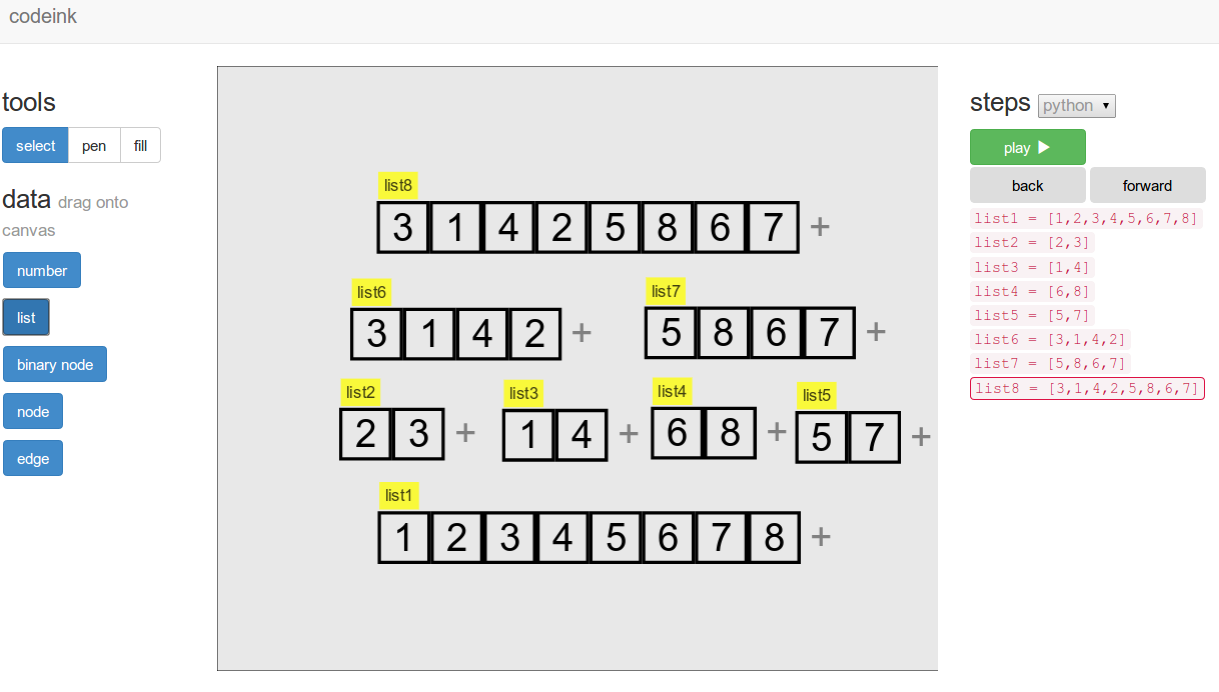
\includegraphics[width=\pagewidth]{mergesort}
%\subsubsection{AVL Insertion}
%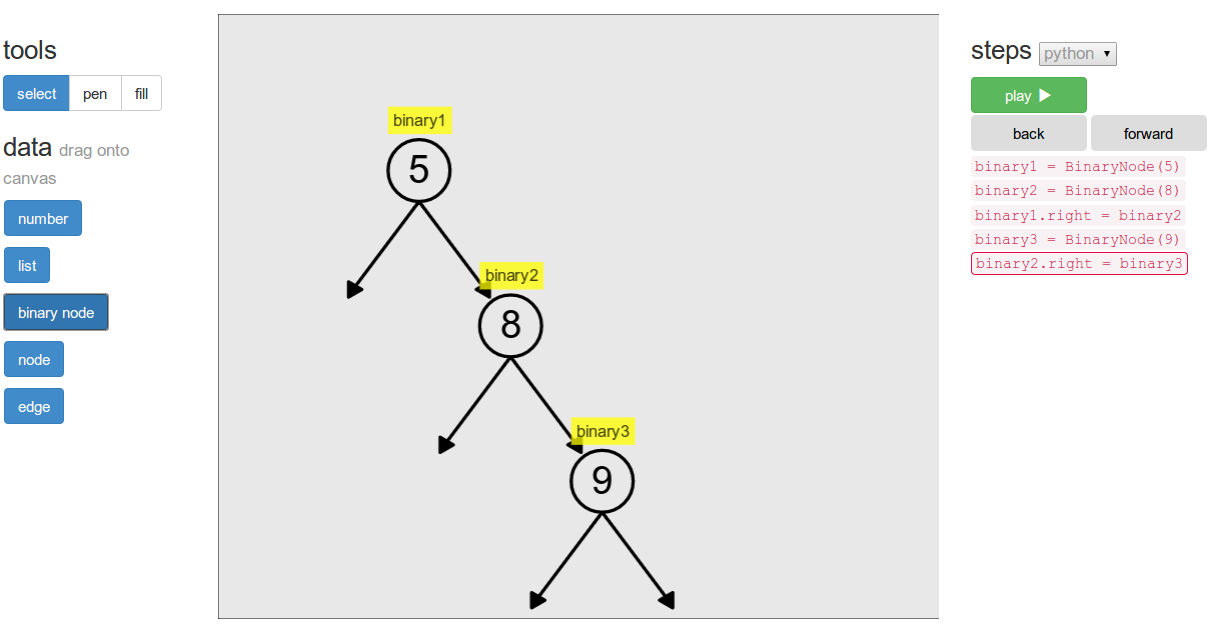
\includegraphics[width=\pagewidth]{BST}
%\subsubsection{Dijkstra's Algorithm}

